% TODO: Modifica immagine
\begin{figure}[h]
    \centering
    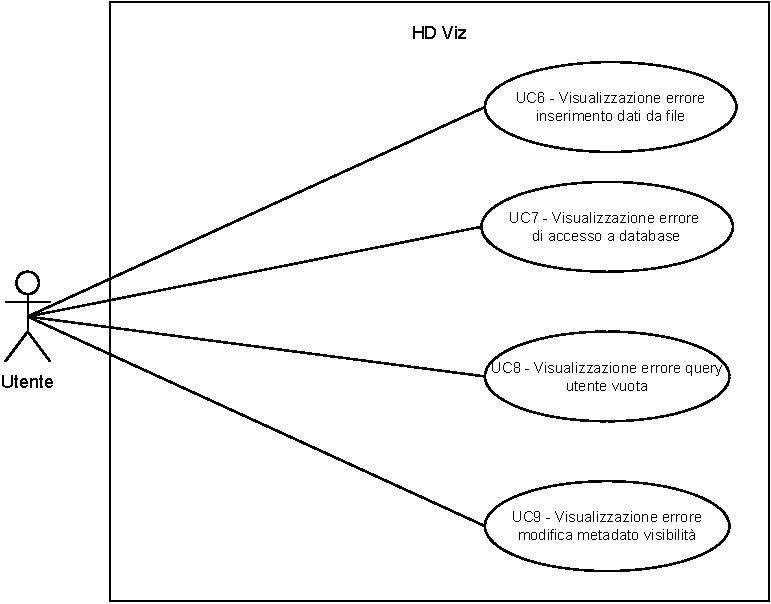
\includegraphics[width=0.7\textwidth]{diagrammi/UC_errori.pdf}
    \caption{Diagramma rappresentante gli use case degli errori}
    \label{fig:UC5}
\end{figure}

%TODO: Cambiare numerazione? Al momento ha senso da una parte ma non è giustificata qui visto che sottocasi non sono veri e propri.

\subsection{UC5 - Visualizzazione errore inserimento dati da file}
\label{sub:uc6}
\begin{itemize}
    \item \textbf{Descrizione}: L'utente visualizza un messaggio di errore dopo aver caricato un file CSV non corretto 
    o vuoto;

    \item \textbf{Attore primario}: Utente;
    
    \item \textbf{Precondizione}:   L'utente carica un file CSV non corretto o vuoto (\hyperref[ssub:uc1.2]{UC1.2});

    \item \textbf{Postcondizione}:  Viene visualizzato un messaggio di errore relativo alla non correttezza del file 
    caricato;

    \item \textbf{Scenario principale}:
    \begin{enumerate}
        \item Viene visualizzato un messaggio d'errore relativo alla non correttezza del file caricato;
        \item L'utente conferma la presa visione dell'errore.
    \end{enumerate}

\end{itemize}


\subsection{UC6 - Visualizzazione errore di accesso a database}
\label{sub:uc7}
\begin{itemize}
    \item \textbf{Descrizione}: L'utente visualizza un messaggio di errore dopo il fallimento dell'accesso
    al database indicato;

    \item \textbf{Attore primario}: Utente;
    
    \item \textbf{Precondizione}:   La connessione con il database indicato dall'utente fallisce 
    (\hyperref[par:uc1.3.1]{UC1.3.1});

    \item \textbf{Postcondizione}:  Viene visualizzato un messaggio di errore relativo al fallimento della connessione 
    con il database indicato dall'utente;

    \item \textbf{Scenario principale}:
    \begin{enumerate}
        \item Viene visualizzato un messaggio d'errore relativo alla mancata connessione al database indicato dall'utente;
        \item L'utente conferma la presa visione dell'errore.
    \end{enumerate}
\end{itemize}


\label{sub:uc8}


\subsection{UC7 - Visualizzazione errore query utente vuota}
\label{sub:uc9}
\begin{itemize}
    \item \textbf{Descrizione}: L'utente visualizza un messaggio di errore per l'esecuzione di una query sul database 
    esterno che ha restituito un dataset non valido;

    \item \textbf{Attore primario}: Utente;
    
    \item \textbf{Precondizione}:   La query eseguita ha restituito un dataset non valido 
    (\hyperref[par:uc1.3.2]{UC1.3.2});

    \item \textbf{Postcondizione}:   Viene visualizzato un messaggio di errore relativo alla restituizione di un dataset non valido dall'esecuzione di una query sul database esterno;
    
    \item \textbf{Scenario principale}:
    \begin{enumerate}
        \item Viene visualizzato un messaggio d'errore relativo relativo alla restituizione di un dataset non valido 
        dall'esecuzione di una query sul database esterno;
        \item L'utente conferma la presa visione dell'errore.
    \end{enumerate}

\end{itemize}

\subsection{UC8 - Visualizzazione errore modifica metadato di visibilità}
\label{sub:uc10}

\begin{itemize}
    \item \textbf{Descrizione}: L'utente visualizza un messaggio di errore per la modifica impropria di un metadato di 
    visibilità;

    \item \textbf{Attore primario}: Utente;
    
    \item \textbf{Precondizione}:   Viene impostato un metadato di visibilità a "nascosta", con meno di due dimensioni 
    visibili;

    \item \textbf{Postcondizione}:   Viene visualizzato un messaggio di errore relativo alla modifica impropria di un 
    metadato di visibilità;

    \item \textbf{Scenario principale}:
    \begin{enumerate}
        \item Viene visualizzato un messaggio di errore relativo alla modifica impropria di un metadato di visibilità;
        \item L'utente conferma la presa visione dell'errore.
    \end{enumerate}
\end{itemize}